%
% kernbildintro.tex
%
% (c) 2021 Prof Dr Andreas Müller, OST Ostschweizer Fachhochschule
%
\bgroup

\definecolor{grueneins}{rgb}{0.0,0.4,0.0}
\definecolor{gruenzwei}{rgb}{0.0,0.4,0.8}
\definecolor{orangeeins}{rgb}{1.0,0.6,0.0}
\definecolor{orangezwei}{rgb}{0.8,0.0,0.4}

\begin{frame}[t]
\frametitle{Bilder und Kerne}
\vspace{-15pt}
\begin{center}
\begin{tikzpicture}[>=latex,thick]

\begin{scope}[xshift=-3.4cm]

\only<1>{
\node at (0,0) {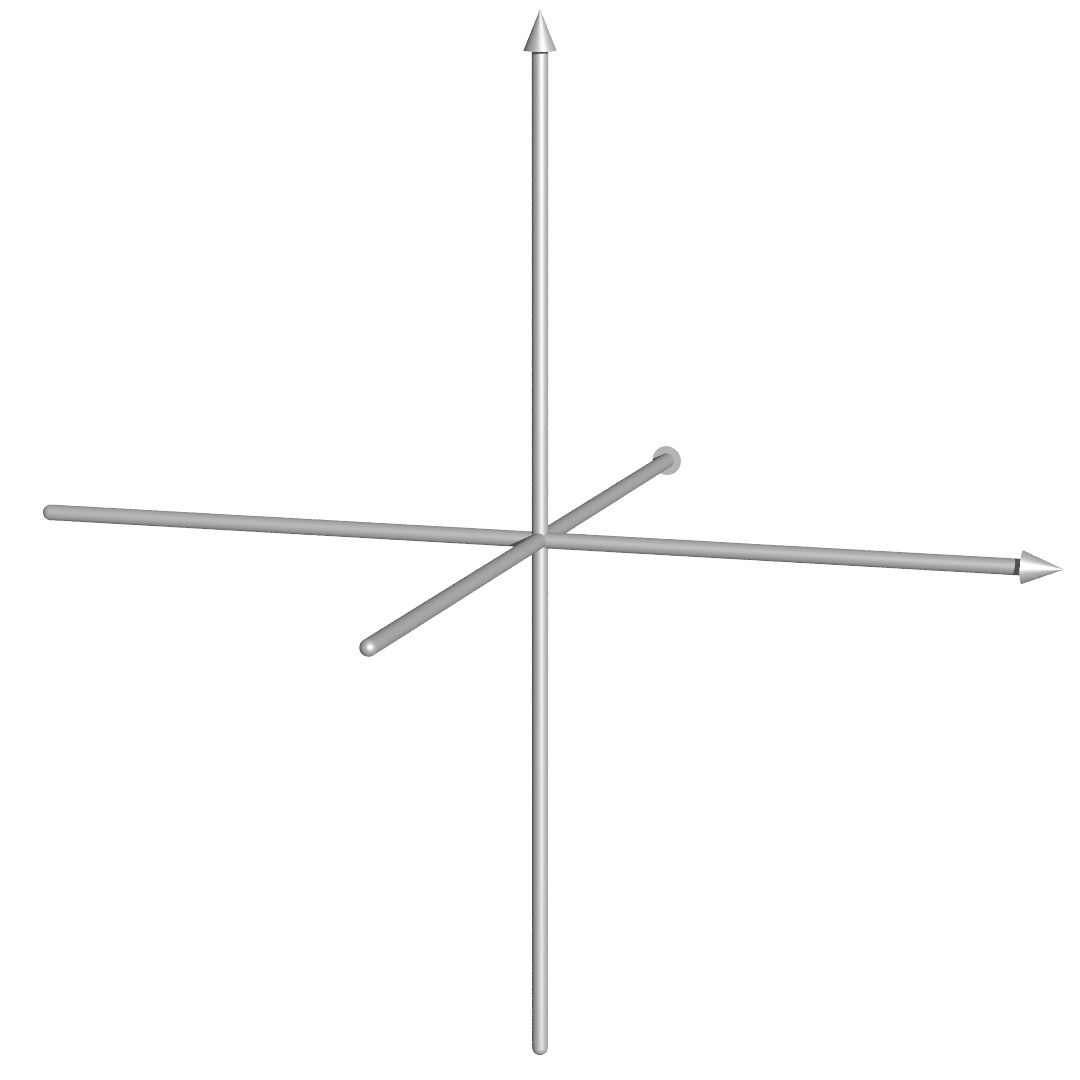
\includegraphics[width=6.6cm]{../slides/5/beispiele/leer.jpg}};
}
\only<2-3>{
\node at (0,0) {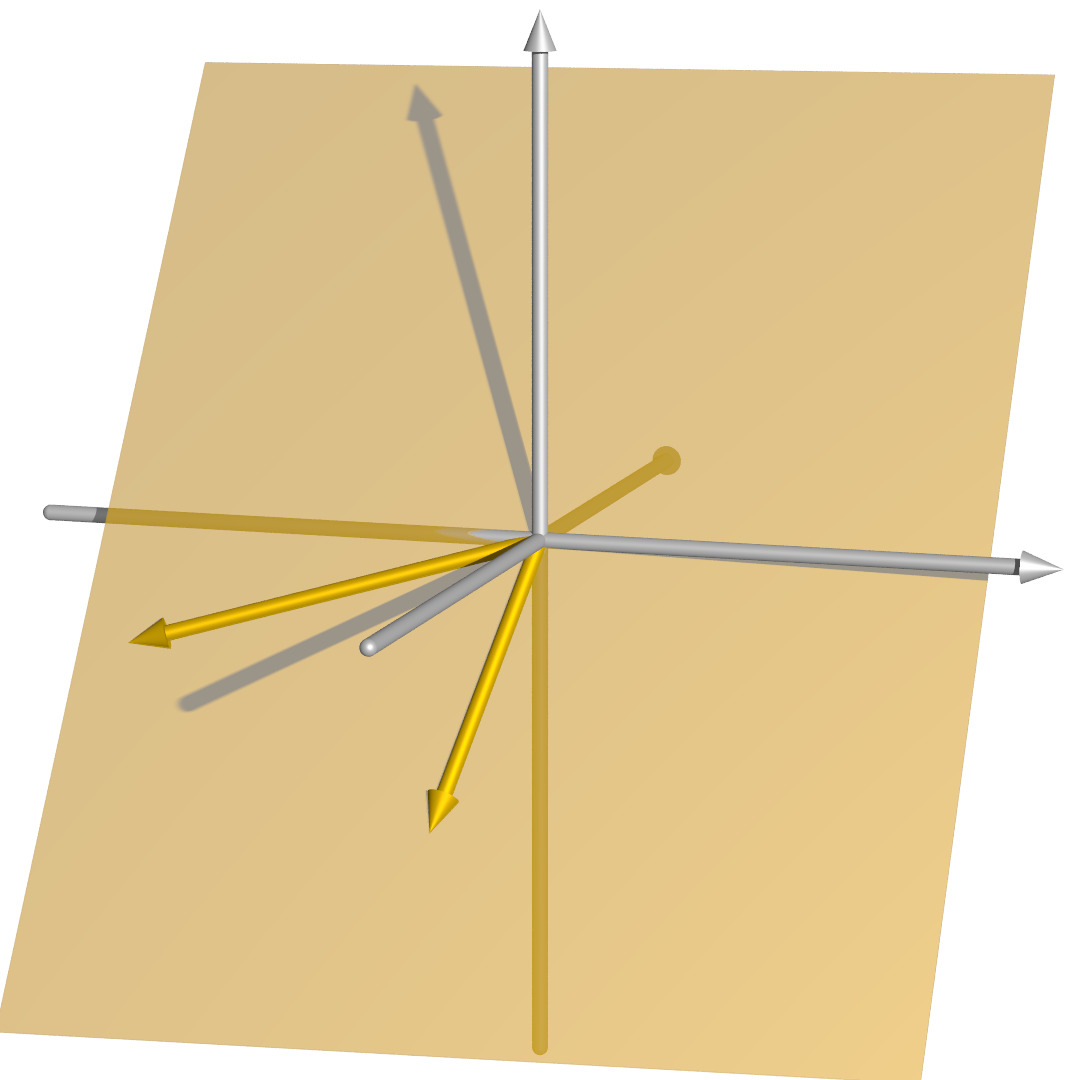
\includegraphics[width=6.6cm]{../slides/5/beispiele/bild1.jpg}};
}
\uncover<4->{
\node at (0,0) {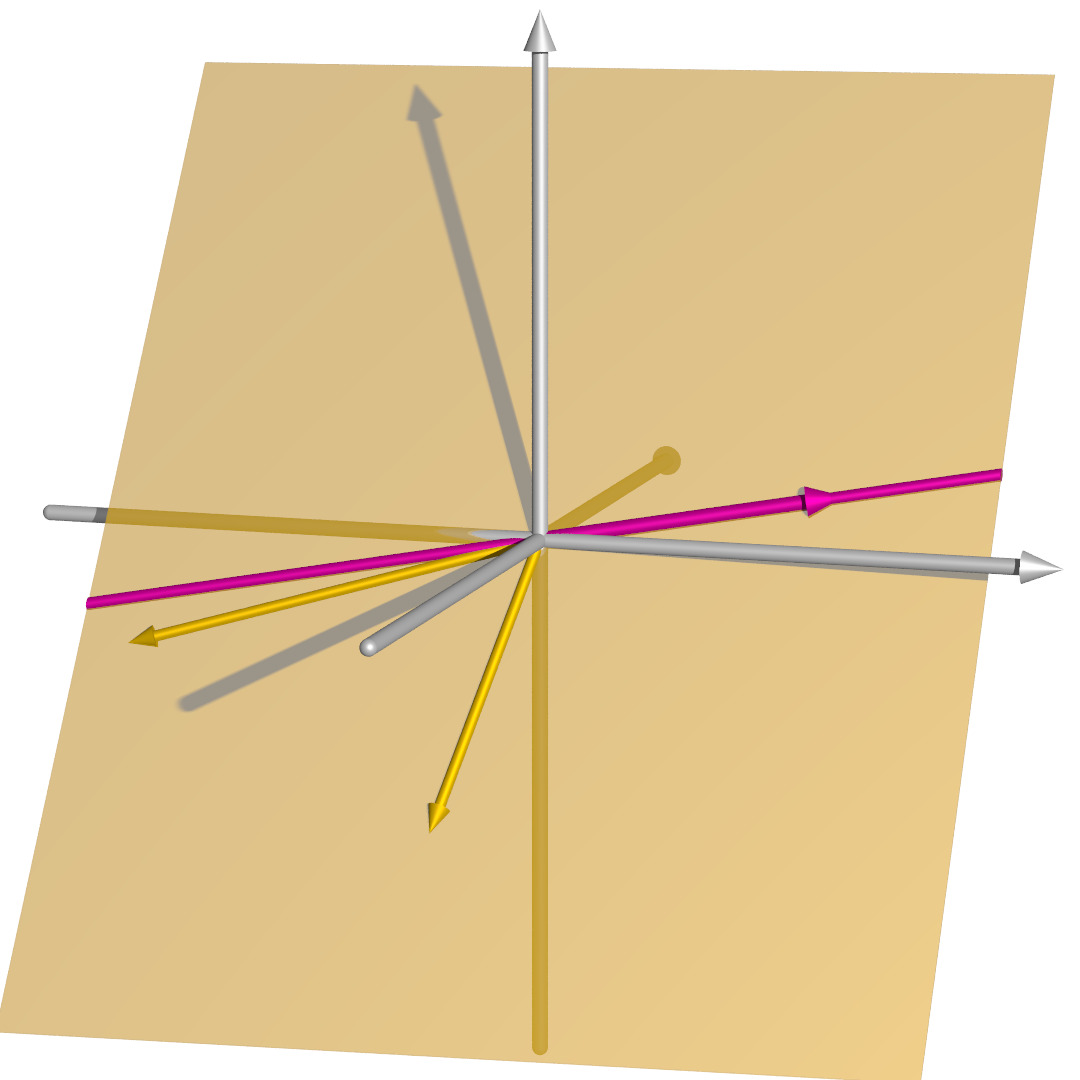
\includegraphics[width=6.6cm]{../slides/5/beispiele/bild2.jpg}};
}
\uncover<2->{
	\fill[color=white,opacity=0.7]  (0.1,2.18) rectangle (4,2.64);
	\node[color=orangeeins] at (0,2.4) [right]
		{$\operatorname{im} A = \{Av\;|v\in\mathbb{R}^n\}$};
}
\uncover<4->{
	\node[color=orangezwei] at (4,0.7) [left]
		{$\operatorname{im} A^2 = \{A^2v\;|v\in\mathbb{R}^n\}$};
}
\end{scope}

\begin{scope}[xshift=3.4cm]

\uncover<2->{
\fill[color=orangeeins!40] (-1,0.5) rectangle (1.8,2);
}
\uncover<4->{
\fill[color=orangezwei!40] (-1.1,-1.7) rectangle (-0.,-0.3);
}

\node at (0,0) {\begin{minipage}{6cm}
\begin{align*}
A&={\scriptstyle\begin{pmatrix*}[r]
  -0.979& -0.142&  0.917\\
  -0.260& -0.643&  1.069\\
  -0.285& -0.449&  0.823
\end{pmatrix*}}
\\
\operatorname{Rang}A&=2
\\
\uncover<3->{
A^2&={\scriptstyle\begin{pmatrix*}[r]
   0.734& -0.181& -0.295\\
   0.118& -0.029& -0.047\\
   0.161& -0.039& -0.065
\end{pmatrix*}}}\\
\uncover<3->{
\operatorname{Rang}A^2&=1}
\end{align*}
\end{minipage}};

\only<5>{
\node at (0,0) {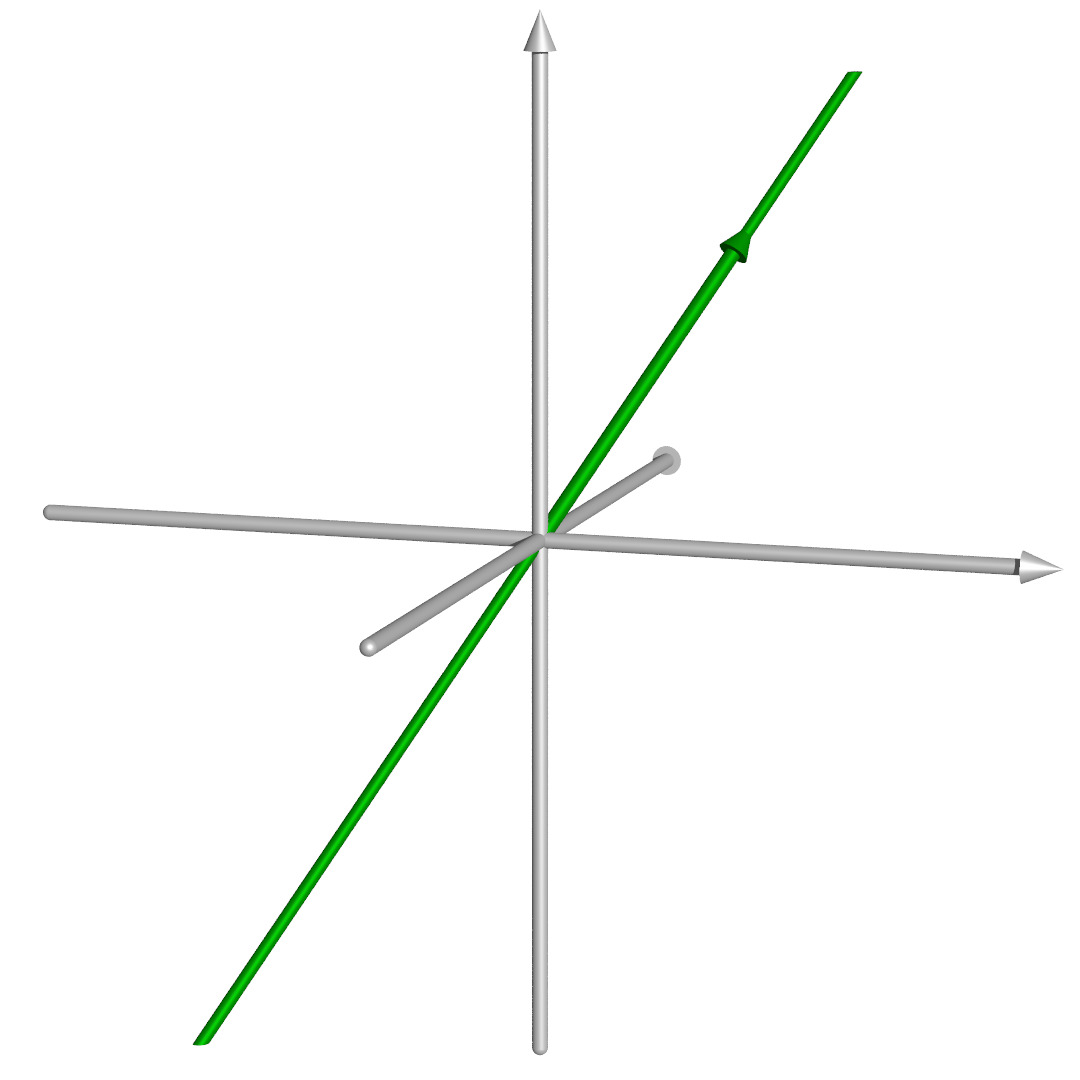
\includegraphics[width=6.6cm]{../slides/5/beispiele/kern1.jpg}};
}

\uncover<6->{
\node at (0,0) {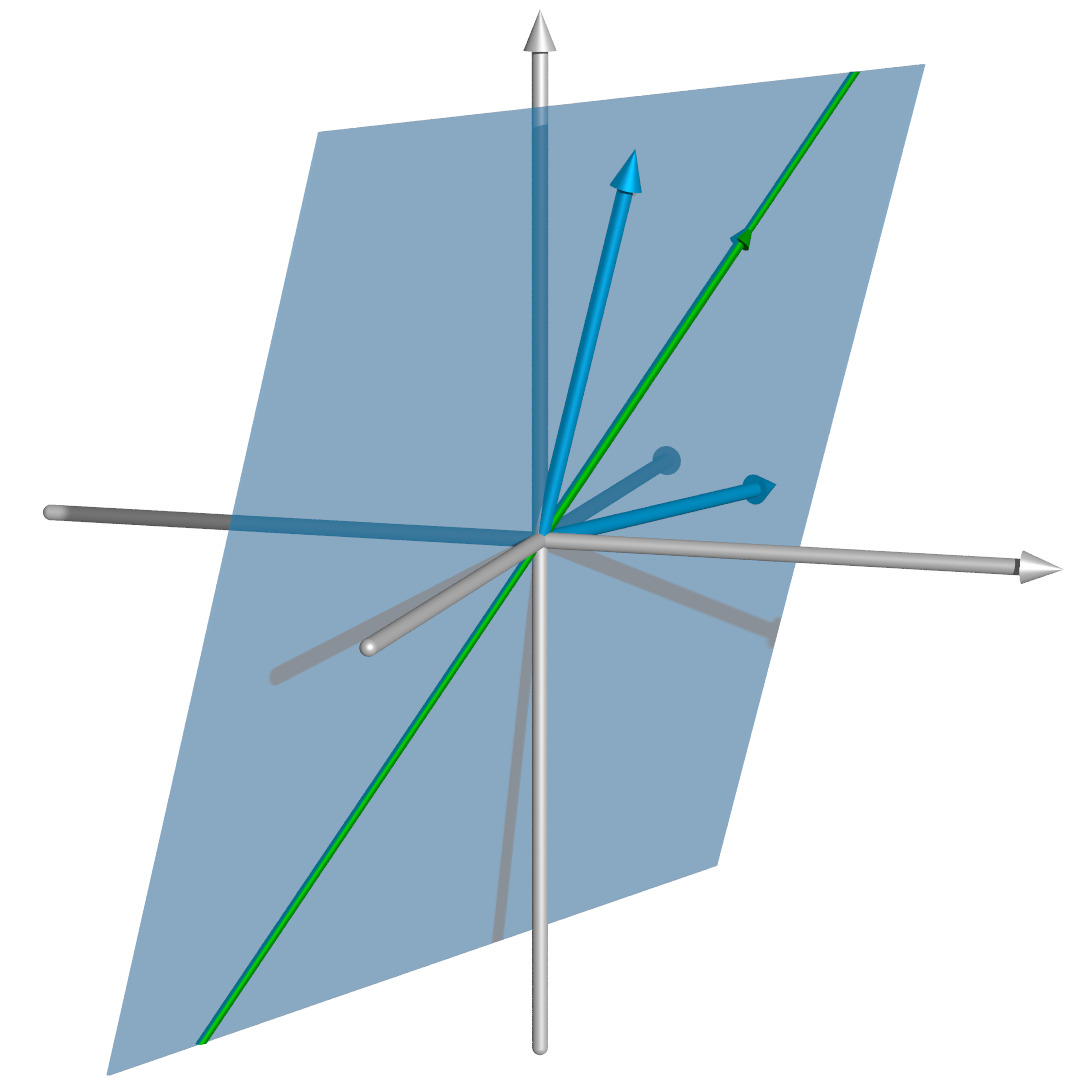
\includegraphics[width=6.6cm]{../slides/5/beispiele/kern2.jpg}};
\node[color=gruenzwei] at (-1.35,-3.0) [right] {$\ker A^2 = \{v\;|\; A^2v=0\}$};
}

\uncover<5->{
\node[color=grueneins] at (-0.9,3.1) [right] {$\ker A = \{v\;|\; Av=0\}$};
}

\end{scope}

\end{tikzpicture}
\end{center}
\end{frame}
\egroup
